\section{方向信息的处理}
\label{sec:opt-sto-direction}

到目前为止，算法实际使用的方向要么是读数本身，要么是读数经过平均或缩放的结果。实践中还有两类更直接的改动：把过大的读数截短，以及在导数没有用处的地方人为指定一个反向传播规则。两者都会让实际方向偏离原目标的梯度。本节先给出操作的定义，再回到原目标检查所得方向的含义：计算图返回了一个向量，并不意味着这个向量是原目标的梯度，也不意味着沿它走一步会下降。

\subsection{梯度裁剪}
\label{sec:opt-sto-clipping}

\paragraph{两种裁剪}
\term{梯度裁剪}（gradient clipping）在读数过大时把它缩短，常用来防止个别巨大读数把参数推得太远，例如循环网络训练中梯度突然爆炸的情形\scite{pascanu2013}。给定阈值$c>0$，有两种做法。逐坐标裁剪把每个坐标截到区间$[-c,c]$内：
\[
  [\operatorname{clip}^{\mathrm{elem}}_c(\bm g)]_k=\max\{-c,\min\{c,g_k\}\};
\]
范数裁剪则整体缩放，只在范数超过阈值时生效：
\[
  \operatorname{clip}_c(\bm g)=\bm g\cdot\min\Bigl\{1,\frac{c}{\lVert\bm g\rVert_2}\Bigr\}.
\]
图~\ref{fig:opt-sto-clipping}(a)对同一个读数$\bm g=(3,4)$、$c=1$比较两者。逐坐标裁剪得到$(1,1)$，范数为$\sqrt2$，方向从与第一坐标轴夹角约$53^\circ$变成$45^\circ$；范数裁剪得到$(0.6,0.8)$，范数为$1$，方向不变。前者把读数投影到边长为$2c$的正方形上，后者投影到半径为$c$的圆盘上。

\paragraph{裁剪的位置}
裁剪放在算法的哪一环，得到的是不同的算法。裁剪原始读数，后续的动量和平方统计看到的是裁过的读数；裁剪经过统计缩放后的方向（Adafactor按均方根裁剪就是这一种），统计仍记录原始读数；裁剪最终位移，则限制的是$\lVert\bm x^{(t+1)}-\bm x^{(t)}\rVert_2$本身。在小批量中，先裁剪每个样本的读数再平均，与先平均再裁剪也不同。描述一个训练过程时必须写明裁剪的对象和阈值。

\paragraph{裁剪带来的偏差}
裁剪是非线性运算，它改变读数的平均。设标量读数以相等概率取$2$与$-1$，均值为$1/2$。用$c=1$裁剪后，读数变为$1$与$-1$，均值为$0$：期望方向消失了。图~\ref{fig:opt-sto-clipping}(b)画出裁剪后均值随阈值的变化：对这个两点分布，$c<1$时均值为$0$，$1\leq c<2$时为$(c-1)/2$，$c\geq2$时恢复为$1/2$；对向一侧拖尾的连续分布$-1+\operatorname{Exp}(1.5)$，均值随$c$平滑上升，但在任何有限阈值下都低于$1/2$。偏差的方向取决于读数分布的形状，不一定指向零。用第~\ref{sec:opt-sto-unbiased}节的分解，裁剪后的读数有非零的条件偏差$\bm\beta^{(t)}$，必须作为偏差处理，不能当作无偏梯度套用前面的定理。

\begin{figure*}[!htbp]
  \centering
  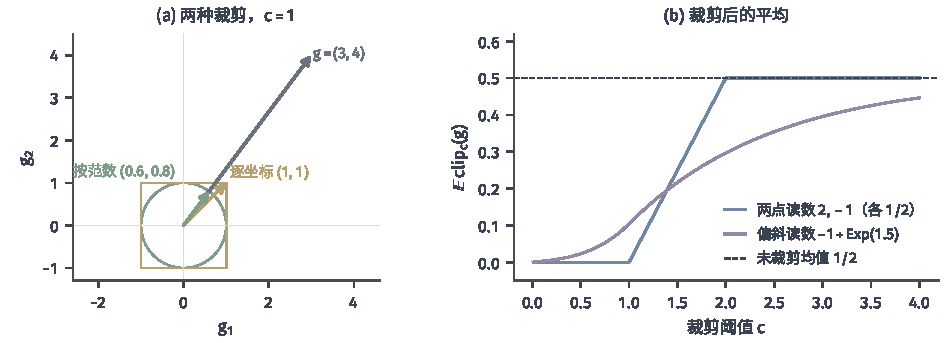
\includegraphics[width=160mm]{figures/03-optimization-evolution-and-signals/01-optimization/matplotlib/c6-clipping/figure.pdf}
  \caption{梯度裁剪的几何与偏差。(a) 读数$\bm g=(3,4)$，阈值$c=1$：逐坐标裁剪落在黄色正方形的角上，得到$(1,1)$；范数裁剪沿原方向缩到绿色单位圆上，得到$(0.6,0.8)$。(b) 标量读数裁剪后的均值$\mathbb E\operatorname{clip}_c(g)$随阈值$c$的变化。蓝线：以相等概率取$2$与$-1$；紫线：$g=-1+E$，$E$服从均值为$1.5$的指数分布。两者未裁剪时均值都是$1/2$（虚线）。}
  \label{fig:opt-sto-clipping}
\end{figure*}

增大批量能否减小这一偏差，取决于裁剪的位置。若逐样本裁剪后再平均，批量平均的是裁过的读数，期望仍是裁剪后的均值，偏差不随批量变小。若先平均再裁剪，批量越大，平均读数越集中在真梯度附近，被裁剪的概率越小；只要真梯度的范数小于阈值，偏差随批量增大而减小。

\paragraph{分别评价三种作用}
裁剪的作用应拆开评价。第一是限制位移：范数裁剪保证每步位移不超过$\eta c$，这是确定的。第二是引入偏差：如上所述，它使期望方向偏离梯度，在误差界中表现为不随步长消失的项，第~\ref{sec:opt-sto-perturbation}节会给出这一项的位置。第三是可能控制噪声：读数分布有重尾、二阶矩很大甚至无穷时，裁剪后的读数二阶矩有界，前面依赖方差假设的分析才有可能使用。是否值得用偏差换取有界的二阶矩，要看具体分布，不存在无条件的结论。

\subsection{离散前向与替代梯度（补充）}
\label{sec:opt-sto-surrogate}

\paragraph{导数处处为零的前向}
量化网络把连续参数取整后再使用。设$Q(w)=\operatorname{round}(w)$，损失$F(w)=\tfrac12(Q(w)-a)^2$。$Q$在非半整数点处局部为常数，所以除了可数个跳跃点外$F'(w)=0$：经典梯度不提供任何关于往哪边走的信息，梯度下降一步也不会动。这与第~\ref{sec:opt-sto-expectation}节的指示函数例同源：前向函数分片常数，信息全部藏在跳跃里。

\paragraph{直通估计}
\term{直通估计}（straight-through estimator）在反向计算时假装$Q$是恒等映射，即人为规定$\mathrm dQ/\mathrm dw=1$\scite{math-bengio2013estimating}，于是返回的方向是$g_{\mathrm{STE}}(w)=Q(w)-a$。这类人为指定的反向信号统称\term{替代梯度}（surrogate gradient）。区分两件事很重要：前向函数$F$是实际被评价的对象，反向规则是我们另外选的方向生成方式，两者之间没有求导关系。用有限差分检查得到的是前向函数的导数（这里是零），不能用来“验证”替代梯度。

图~\ref{fig:opt-sto-ste}给出同一点出发的两个结果。取$w=0.2$，$Q(w)=0$。若$a=1$，$F=0.5$，替代梯度为$-1$；取步长$0.4$走到$w=0.6$，$Q=1$，损失降为$0$。若$a=0.4$，$F=0.08$，替代梯度为$-0.4$；取步长$1$同样走到$w=0.6$，损失却升到$0.18$：$Q$跳过了目标$0.4$，落在另一侧更远的整数上。光滑下降的证明依赖于“小步之内一阶模型准确”，而跨过跳跃点时一阶模型完全失效，因此无法从替代梯度推出下降。

\begin{figure}[!htbp]
  \centering
  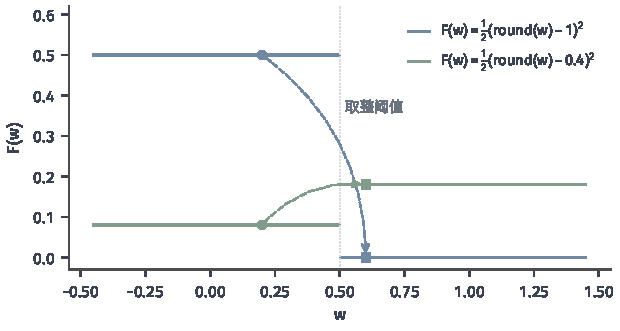
\includegraphics[width=105mm]{figures/03-optimization-evolution-and-signals/01-optimization/matplotlib/c6-ste/figure.pdf}
  \caption{取整前向上的直通估计。蓝线$F(w)=\tfrac12(\operatorname{round}(w)-1)^2$，绿线$F(w)=\tfrac12(\operatorname{round}(w)-0.4)^2$，两者都是分段常数，经典导数几乎处处为零；点线为取整阈值$w=0.5$。圆点为起点$w=0.2$，方块为沿替代梯度$\operatorname{round}(w)-a$走一步后的位置$w=0.6$：蓝色（步长$0.4$）损失由$0.5$降到$0$，绿色（步长$1$）损失由$0.08$升到$0.18$。}
  \label{fig:opt-sto-ste}
\end{figure}

\paragraph{替代方向的地位}
替代梯度一般既不是经典梯度，也不是次梯度。以$a=1$、$w=0.2$为例：要求$F(y)\geq F(w)+s(y-w)$对一切$y$成立的斜率$s$并不存在，因为$y=0.6$处要求$s\leq-1.25$，$y=-0.4$处（$F$仍为$0.5$）要求$s\geq0$；只看局部时$F$在该点附近为常数，局部意义下的次梯度只有$0$。替代梯度$-1$两者都不是。所以训练是否成功只能回到实际的前向任务上评价：比较前向损失、验证指标或原问题的目标值，而不是看替代梯度的范数是否变小。停止准则也应基于前向量。

\paragraph{向量量化与停止梯度}
\term{向量量化}（vector quantization）把编码器输出$\bm z$替换为码本中最近的向量$\bm e_{k^\star}$，$k^\star=\argmin_k\lVert\bm z-\bm e_k\rVert_2$，选择最近者也是分段常数的运算。常见做法用一个\term{停止梯度}（stop-gradient）标记$\operatorname{sg}$写成$\bm z_q=\bm z+\operatorname{sg}(\bm e_{k^\star}-\bm z)$\scite{nlp-speech-oord2017vqvae}：前向时$\operatorname{sg}$原样传值，所以$\bm z_q=\bm e_{k^\star}$；反向时$\operatorname{sg}$阻断传播，所以对$\bm z$的反向信号相当于单位Jacobian，编码器得到的是直通方向。码本向量本身收不到这条路径的信号，必须另行规定更新，例如在损失中加入$\lVert\operatorname{sg}(\bm z)-\bm e_{k^\star}\rVert_2^2$，或用编码器输出的移动平均更新码本。需要注意，$\operatorname{sg}$是计算图上的传播规则，不是一个普通函数：不存在一个函数既处处等于恒等映射又导数为零。把它当作函数去求导或分析，会得到自相矛盾的结论。
